\chapter{Les fractales}
\label{chapter:fractales}
Les fractales sont très liée au chaos, ont retrouve souvent des formes fractales dans les système au comportement chaotique, mais avant de faire le lien avec les parties précédente définission rapidement ce qu'est une fractale: En mathématique une fractale est un objet qui présente une structure similaire indépendament de sont échelle, autrement dit une structure sur laquelle ont peut zoomer indéfiniment et retrouvé la structure de départ. De nombreux objets de formes fractales aproximative sont présent dans la nature, les fougères, les brocolis, les flocons de neige ou les arbres par exemple sont des objets "autosimilaires" sur une échelle étendu mais finie. Il est également possible de généré des formes fractracles à l'aide d'algorithme, l'exemple classique est l'enssemble de Mandelbroat qui est définie comme l'ensemble des points $c$ du plan complexe définie par récurence par\\
\[
    \left\{
    \begin{array}{rcl}
        z_0&=&0\\
        z_{n+1}&=&z_{n}^2+c
    \end{array}
    \right.
\]\\
Les images de l'ensemble de Mandelbrot sont réalisées en parcourant les nombres complexes sur une région carrée du plan complexe et en déterminant pour chacun d'eux si le résultat tend vers l'infini ou pas lorsqu'on y itère une opération mathématique. On obtient alors le graphique suivant:

\begin{figure}[!ht]
    \centering
    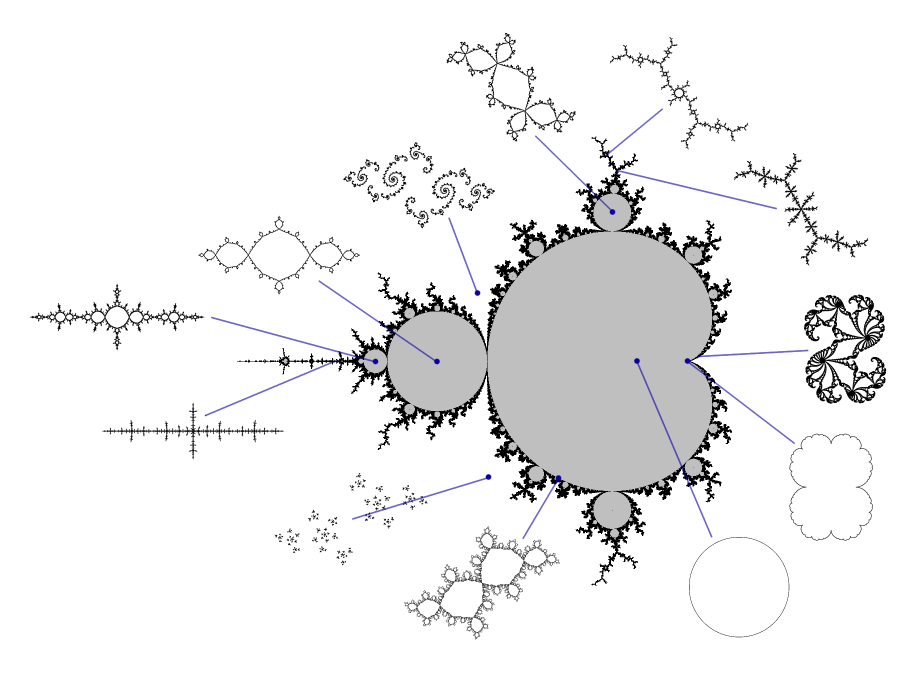
\includegraphics[width=0.5\textwidth]{mandel.png}
    \caption{\label{fig:mandel} Ensemble de Mandelbrot} 
\end{figure}

En zoomant on constate la dimension fratacle, un patern qui se répète a l'infini.


\section{Fractale d'un diagramme de bifurcation}

\section{Fratacle de l'attracteur de Lorenz}
Le cas de l'attracteur de Lorenz est particulié en ce qui concerne les fractales car ça dimension fractale n'est pas directement observable sur ça représentation graphique, la première preuve de sa dimension fractale à été faite purement mathématiquement et ça première observation a été possible en traçant l'attracteur et en concervant 100 chiffre apès la virgule.